\chapter{Progettazione del sistema}
Partendo dai risultati ottenuti nel capitolo precedente, in questo capitolo verrà mostrato come viene strutturata l'architettura del sistema. Ogni entità del diagramma ER corrisponde ad una tabella nel modello relazionale.\cite{DB} Ad ogni tabella corrisponde un modello, secondo il pattern MVC, sul quale saranno effettuate le operazioni \emph{CRUD} (\emph{Create, Read, Update, Destroy}) su richiesta dei controller che attendono istruzioni da parte degli utenti del sistema.\\

Si parte dalla progettazione logica, che prevede una ristrutturazione dello schema ER perché possa avvicinarsi alla realizzazione fisica della base di dati ottenendo lo schema logico, traducibile in schema relazionale. Avviene poi la mappatura delle varie componenti del sistema dullo schema relazionale.\\

\section{Progettazione logica}
\subsection{Ristrutturazione dello schema ER}
Lo schema ER di partenza è molto semplice; non sono presenti ridondanze, cicli, attributi composti, ISA o generalizzazioni, quindi l'unica cosa da fare è quella di individuare gli identificatori principali per ogni entità e relazione\footnote{Per situazioni non ambigue l'identificatore principale non è indicato} aggiungendo in particolare l'attributo \emph{user id} (che ha come dominio i numeri interi) all'entità Giocatore, rendendo così più semplice la realizzazione del database. Non ci sono ulteriori vincoli esterni. Non sono da eseguire altre operazioni.\\

Il risultato della ristrutturazione è nella seguente figura, subito seguita dallo schema relazionale del database.

\begin{figure}[hbt!]
    \centering
    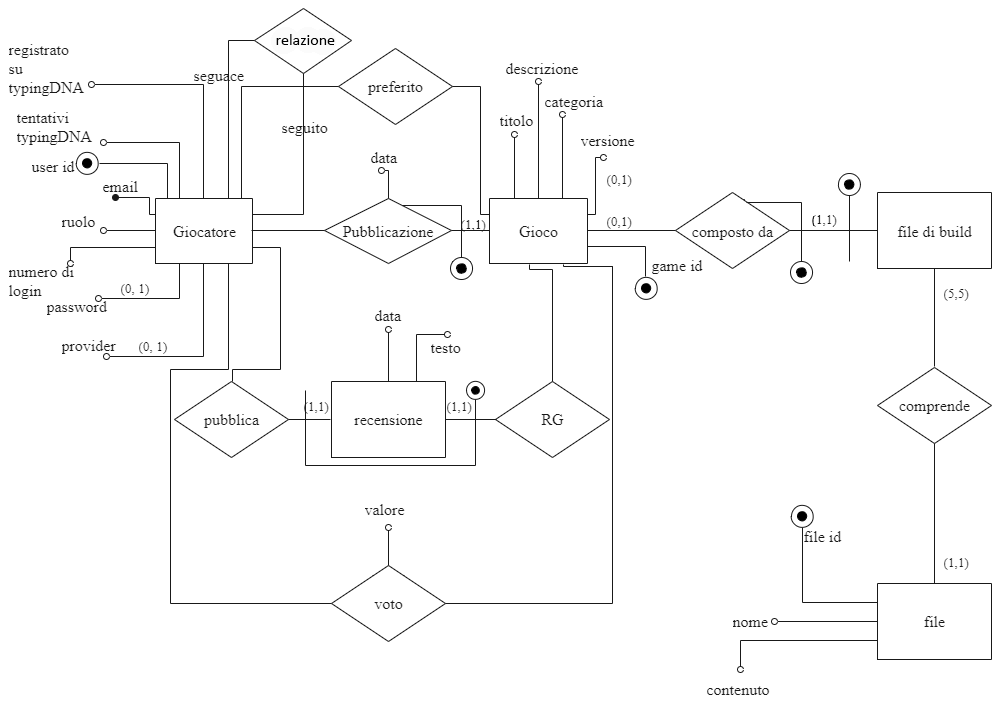
\includegraphics[angle=-90, width=\textwidth]{schemaER_ristrutturato}
    \caption{Schema ER ristrutturato}
\end{figure}

\begin{figure}[hbt!]
    \centering
    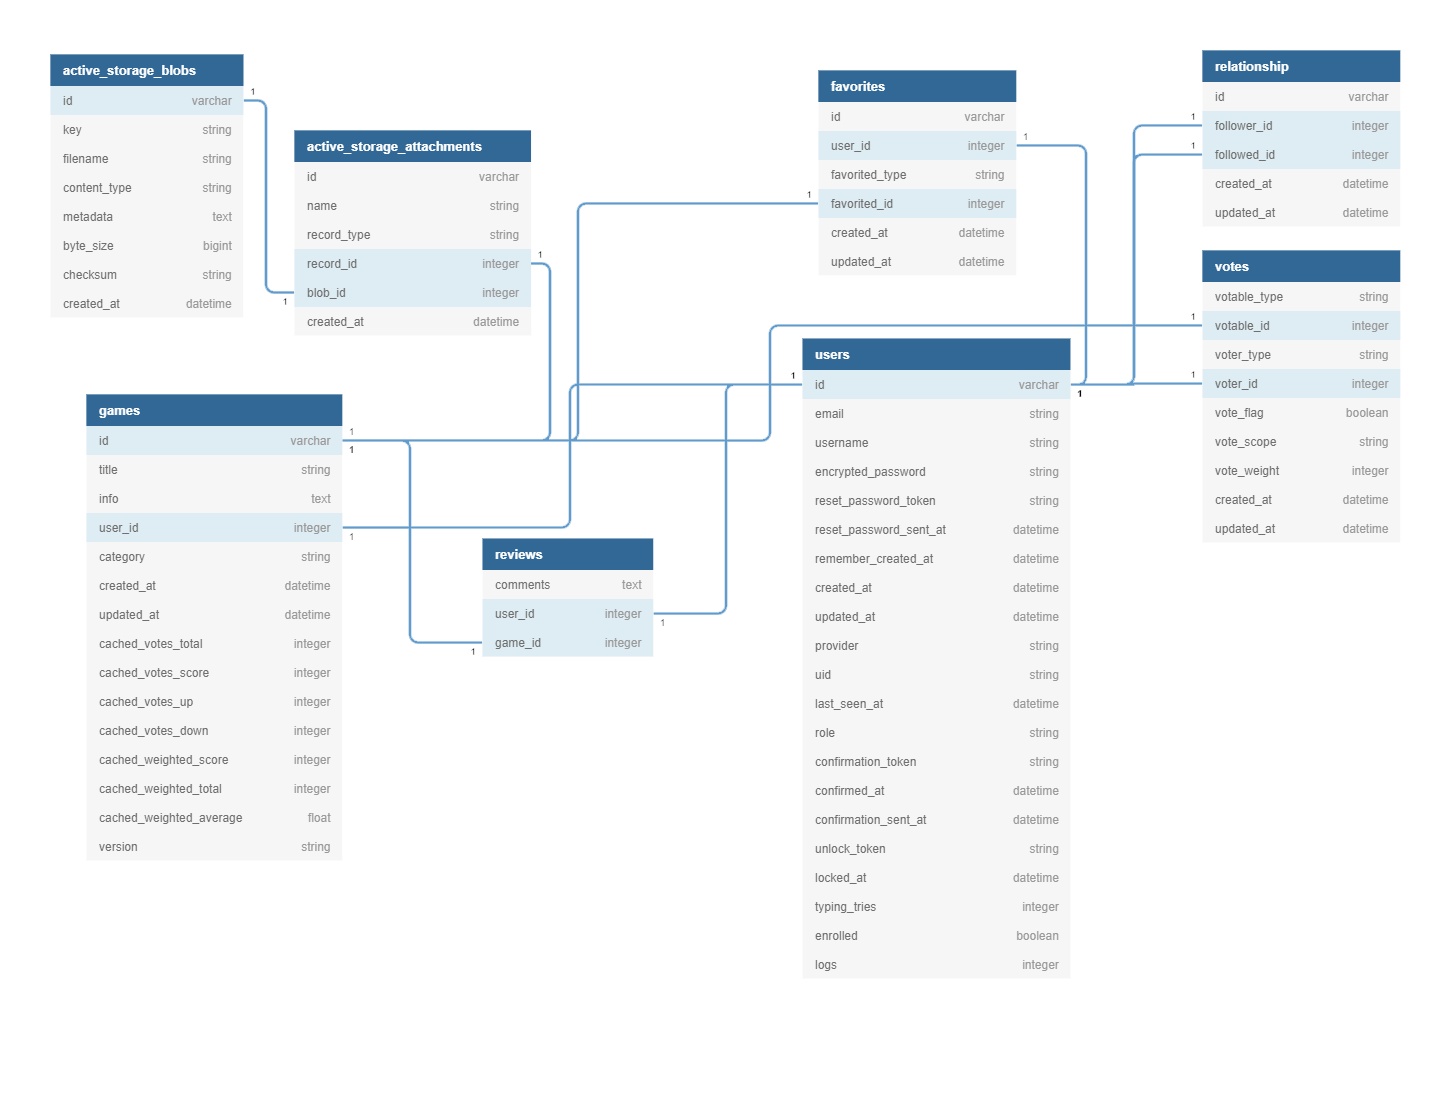
\includegraphics[angle=-90, width=\textwidth]{schema_relazionale}
    \caption{Schema relazionale}
\end{figure}

\FloatBarrier
\section{Architettura dell'applicativo software}
L'approccio \emph{Model-View-Controller} si presta alla realizzazione di applicativi web.\cite{ProgSoft} L'applicazione viene divisa in tre parti: modelli (che si occupano di memorizzare e stabilire le regole sui dati), viste (che presentano i dati e le operazioni disponibili agli utenti) e controllori (che fa da intermediario tra modelli, viste e utente finale), permettendo così di isolare il codice che gestisce i dati da quello che li presenta agli utenti.\\

\subsection{Gestione dei dati}
Per poter memorizzare i dati in un database SQL e contemporaneamente usare l'architettura MVC è necessario collegare le due realtà attraverso librerie di tipo \emph{Object-Relational Mapping} (ORM).\\

Grazie a queste librerie è possibile assegnare ad ogni tabella una classe, ad ogni riga un oggetto della classe, ai valori delle colonne gli attributi degli oggetti. Le query da effettuare sul DB vengono invocate attraverso metodi forniti dalle classi.\\

La seguente immagine mostra il diagramma delle classi per l'applicazione. Ad ogni classe corrisponde un modello.\\

\begin{figure}[hbt!]
    \centering
    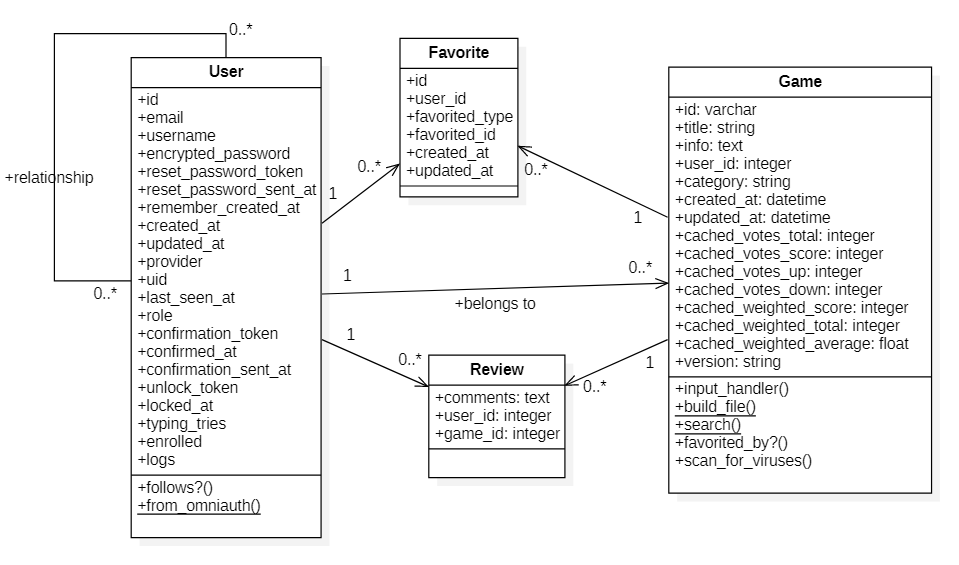
\includegraphics[width=\textwidth]{UML.png}
    \caption{Diagramma UML}
\end{figure}

\FloatBarrier
\subsection{Logica dell'applicazione e presentazione}
Come accennato in precedenza, la logica dell'applicazione viene gestita dai controllori. I controllori recuperano i dati dai modelli e li forniscono alle viste per accessi in lettura, viceversa per modifiche ai dati\footnote{Occorre tenere presente che la vera e propria modifica ai dati viene effettuata dai modelli. I controllori comunicano solo cosa fare.}.\\

Di seguito sono riportati i vari schemi che mostrano come i vari controllori comunicano alle viste i dati da presentare prendendoli dai modelli\footnote{Questi schemi, anche se hanno a che fare con l'architettura vera e propria, intendono essere molto astratti, per rendere la loro lettura il più semplice possibile. La comunicazione, infatti, tra modelli, controllori e viste è più complessa e sotto certi aspetti la lettura diretta del codice renderebbe meglio l'idea.}. Le frecce continue rappresentano la provenienza dei dati dai modelli alle viste attraverso i controllori. Le frecce tratteggiate servono ad indicare una derivazione di un controllore rispetto ad un altro. Dato che tutti i controllori estendono l'\emph{application controller} le frecce tratteggiate corrispondenti sono sottintese. Per semplicità non sono stati inseriti negli schemi i controllori intermediari relativi alla gemma \emph{devise}.

\begin{figure}[hbt!]
    \centering
    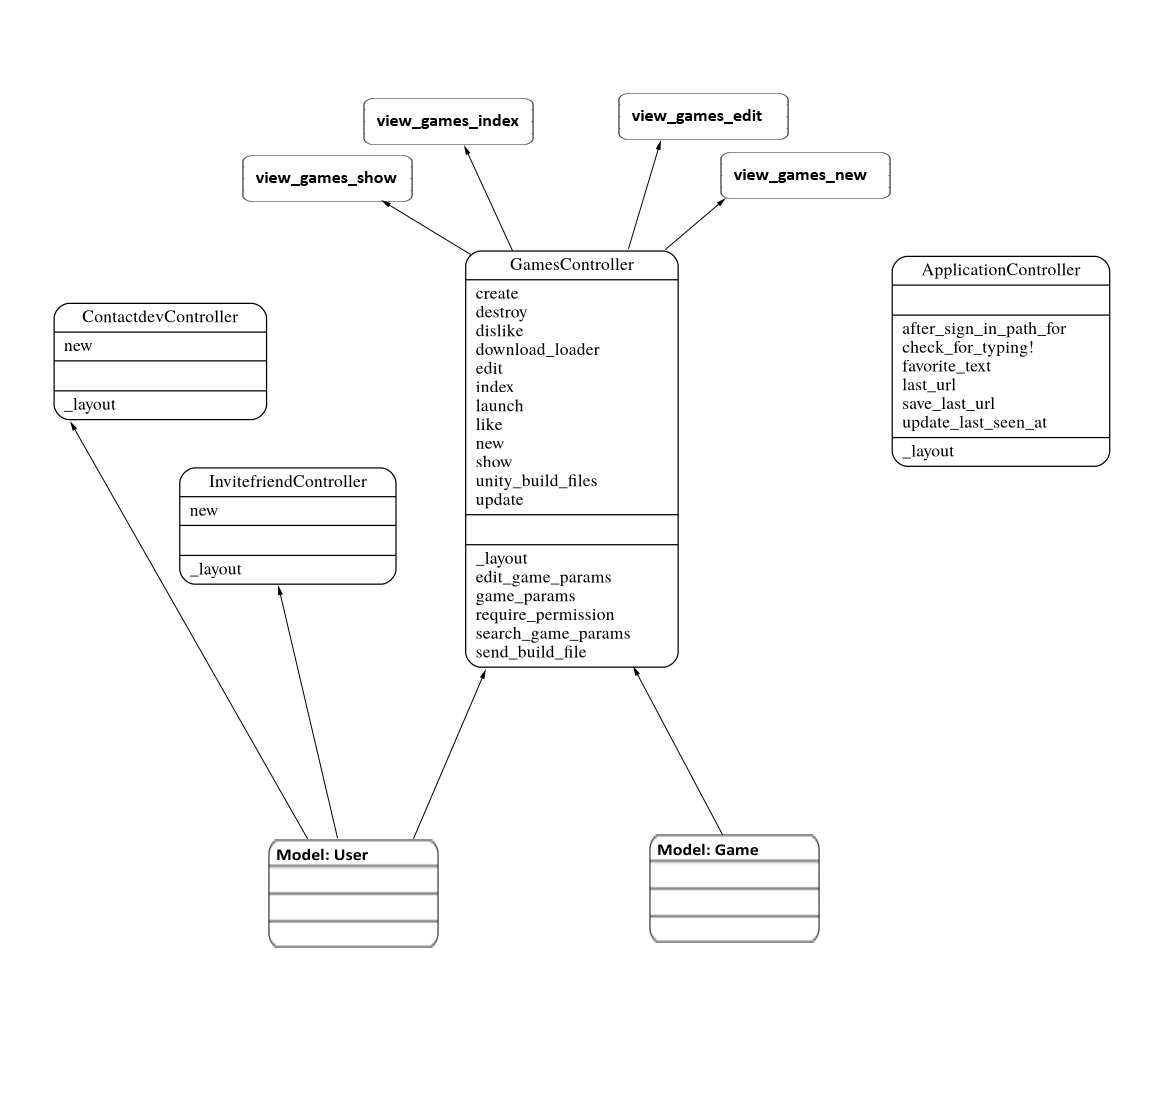
\includegraphics[width=\textwidth]{games_controller.png}
    \caption{GamesController}
\end{figure}

\begin{figure}[hbt!]
    \centering
    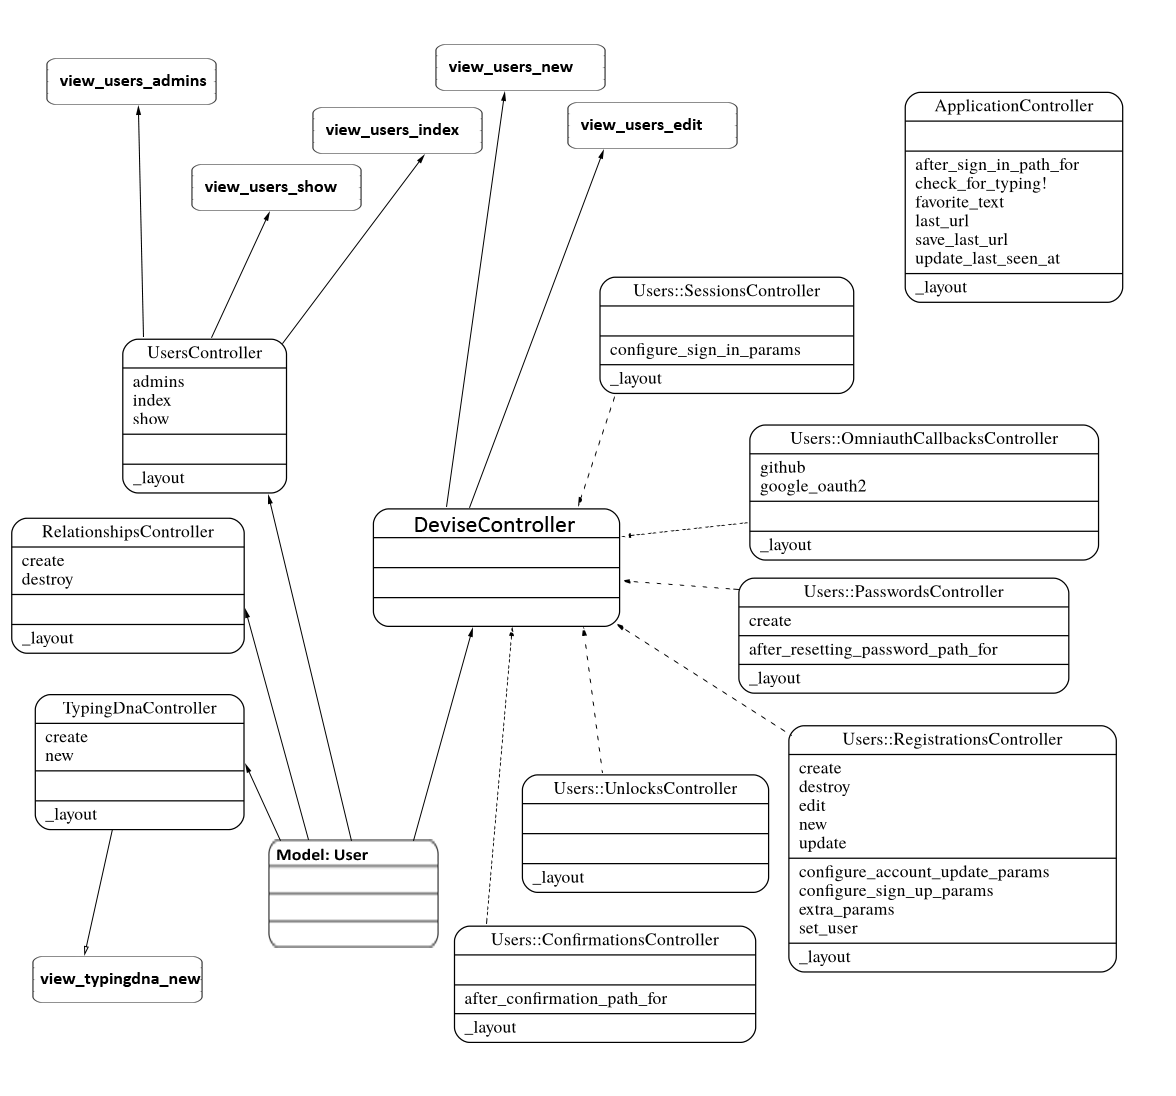
\includegraphics[width=\textwidth]{users_controller.png}
    \caption{UsersController}
\end{figure}
\FloatBarrier
\footnote{\emph{view\_users\_edit} è da intendersi come comprensiva di tutte le viste che presentano campi per modificare gli utenti.}

\begin{figure}[hbt!]
    \centering
    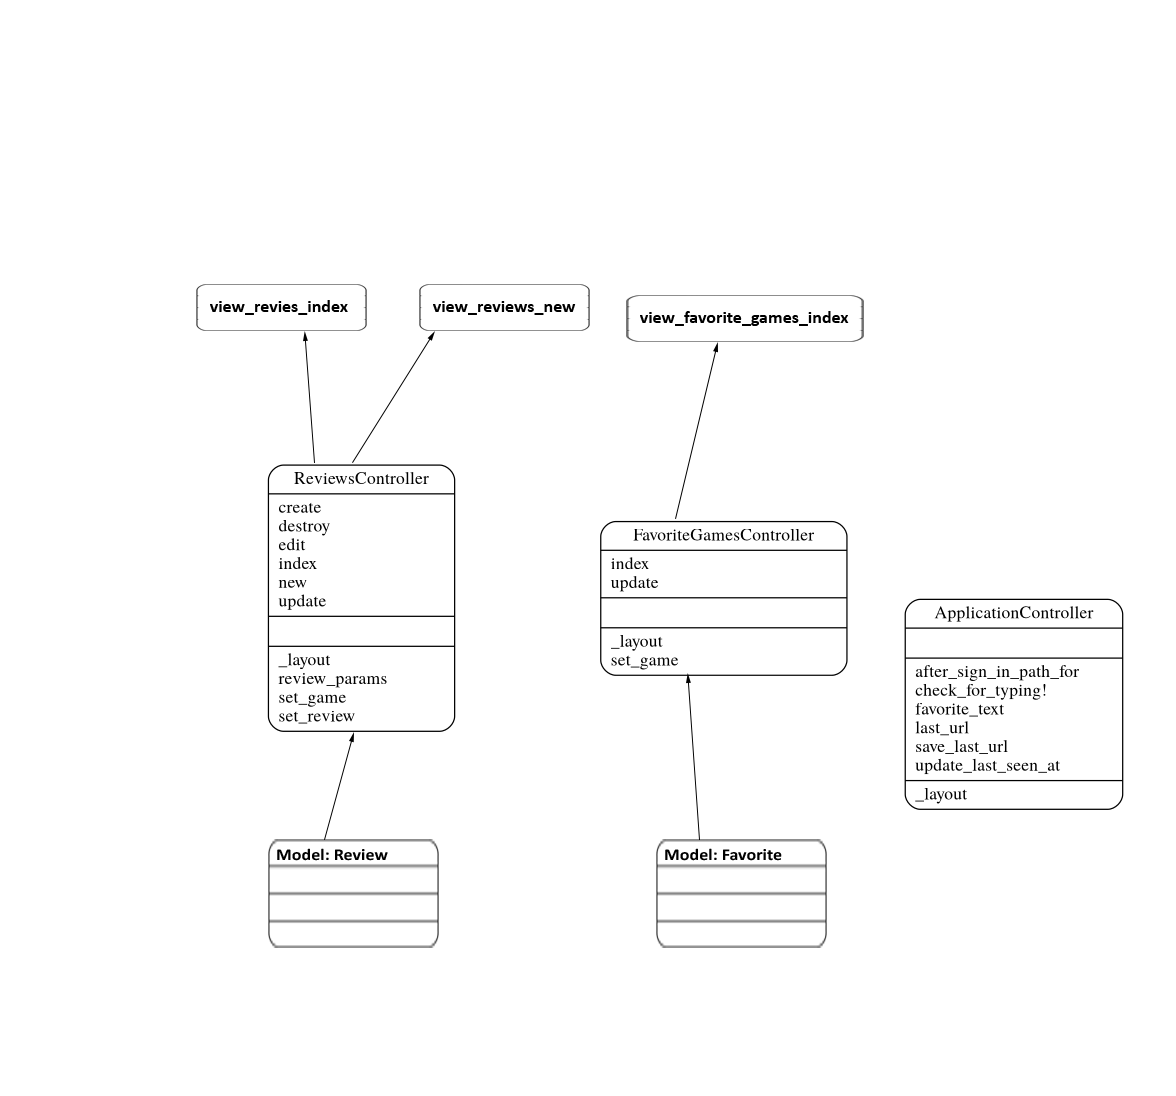
\includegraphics[width=\textwidth]{reviews_favorites_controller.png}
    \caption{ReviewsController e FavoriteGamesController}
\end{figure}